\documentclass{elsarticle}
\usepackage[a4paper,left=2.5cm,right=1.5cm,top=1.5cm,bottom=1.5cm]{geometry}
\usepackage{cite}
\usepackage{amsmath,amssymb,amsfonts,amsthm}
\usepackage{mathtools}
\usepackage[french]{babel}
\usepackage{bm}
\usepackage{algorithmic}
\usepackage{graphicx}
\usepackage{textcomp}
\usepackage{xcolor}
\usepackage{hyperref}
\usepackage{float}
\usepackage[T1]{fontenc}
\usepackage[utf8]{inputenc}
\usepackage{subcaption}
\usepackage{listings}
\usepackage{../../dafny}
\lstset{language=dafny}
\graphicspath{{img/}}
\usepackage{svg}

\makeatletter
\def\ps@pprintTitle{%
	\let\@oddhead\@empty
	\let\@evenhead\@empty
	\def\@oddfoot{\centerline{\thepage}}%
	\let\@evenfoot\@oddfoot}
\makeatother

\makeatletter
\def\blfootnote{\gdef\@thefnmark{}\@footnotetext}
\makeatother

\def\BibTeX{{\rm B\kern-.05em{\sc i\kern-.025em b}\kern-.08em
		T\kern-.1667em\lower.7ex\hbox{E}\kern-.125emX}}
\newcommand{\abs}[1]{\left\lvert#1\right\lvert}
\usepackage{siunitx}
\begin{document}
\title{Méthodes de conception de programmes \\ Devoir 1: Preuve de programme}
\date{12 mars 2019}

\address[add1]{École Polytechnique, Université catholique de Louvain, Place de l'Université 1, 1348 Ottignies-Louvain-la-Neuve, Belgique}

\author[add1]{Alexandre \textsc{Gobeaux}}
\ead{alexandre.gobeaux@student.uclouvain.be}

\author[add1]{Louis \textsc{Navarre}}
\ead{navarre.louis@student.uclouvain.be}

\author[add1]{Gilles \textsc{Peiffer}}
\ead{gilles.peiffer@student.uclouvain.be}

\begin{abstract}
Ce document donne un algorithme pour résoudre le problème 2SUM ainsi qu'une preuve de correction totale pour celui-ci, par rapport aux spécifications définies.
\end{abstract}
\maketitle

\section{Description du problème et de la solution}
Le problème à résoudre est celui d'une séquence d'entiers triée $a$ dans laquelle il faut déterminer si oui ou non deux entrées définies par ces entiers (potentiellement deux fois la même) ont une somme égale à un entier prédéfini $s$.
Si oui, alors le programme doit renvoyer \og \inlinedafny{true} \fg, ainsi que les indices des deux entiers qui satisfont la condition, sinon il renvoie \og \inlinedafny{false} \fg, et la valeur des indices n'a pas d'importance.\blfootnote{\emph{NOMAs$\!\!$:} 42191600 (Alexandre \textsc{Gobeaux}), 12351600 (Louis \textsc{Navarre}), 24321600 (Gilles \textsc{Peiffer})}

Notre algorithme fonctionne en temps linéaire ($\mathcal{O}(n)$), en utilisant deux pointeurs:
le premier commence au premier élément du tableau, alors que le deuxième commence à la fin.
On évalue leur somme à chaque itération, tant que le premier pointeur est plus bas ou équivalent au second:
\begin{itemize}
	\item si celle-ci est plus petite que $s$, on avance d'une unité le premier pointeur;
	\item si celle-ci est plus grande que $s$, on recule d'une unité le deuxième pointeur et
	\item si celle-ci est égale à $s$, on retourne la valeur des indices ainsi que la valeur \og \inlinedafny{true}\fg.
\end{itemize}
L'algorithme peut donc se terminer de deux façons: soit il trouve une paire d'indices qui satisfait la condition, passant donc dans la troisième possibilité ci-dessus,
soit un pointeur dépasse l'autre, ce qui signifie que la séquence ne contient pas de paire satisfaisant la condition.

\section{Spécifications formelles}
\subsection{Précondition}
La précondition est que la séquence soit triée.
Formellement, on demande que
\[
\forall k, \ell \mid 0 \le k \le \ell < \abs{a} :: a[k] \le a[l]\,.
\]
\subsection{Modifie}
L'algorithme ne modifie rien.
\subsection{Postcondition}
La première postcondition est, informellement, que si la valeur booléenne est vraie,
alors $i$ et $j$ contiennent les bonnes valeurs d'indices.
La seconde postcondition est que si la valeur booléenne est fausse,
alors la somme de toute paire est différente de $s$ et que si la somme est différente de $s$ pour toute paire, alors la valeur booléenne retournée est fausse.
Formellement (en appelant \inlinedafny{found} la valeur booléenne),
\begin{align*}
&\textnormal{\inlinedafny{found}} \implies (0 \le i \le j < \abs{a}) \land (a[i] + a[j] = s) \\
\land \lnot &\textnormal{\inlinedafny{found}} \iff \forall m, n \mid 0 \le m \le n < \abs{a} :: a[m] + a[n] \ne s\,.
\end{align*}

\section{Implémentation}
L'implémentation de l'algorithme donné précédemment en Dafny est la suivante.
\lstfile{../src/find_sum.dfy}

\section{Graphe d'exécution}
Le graphe d'exécution pour l'algorithme ci-dessus est donné sur la \textsc{Figure}~\ref{fig:execgraph}.
\begin{figure}[htbp]
	\centering
	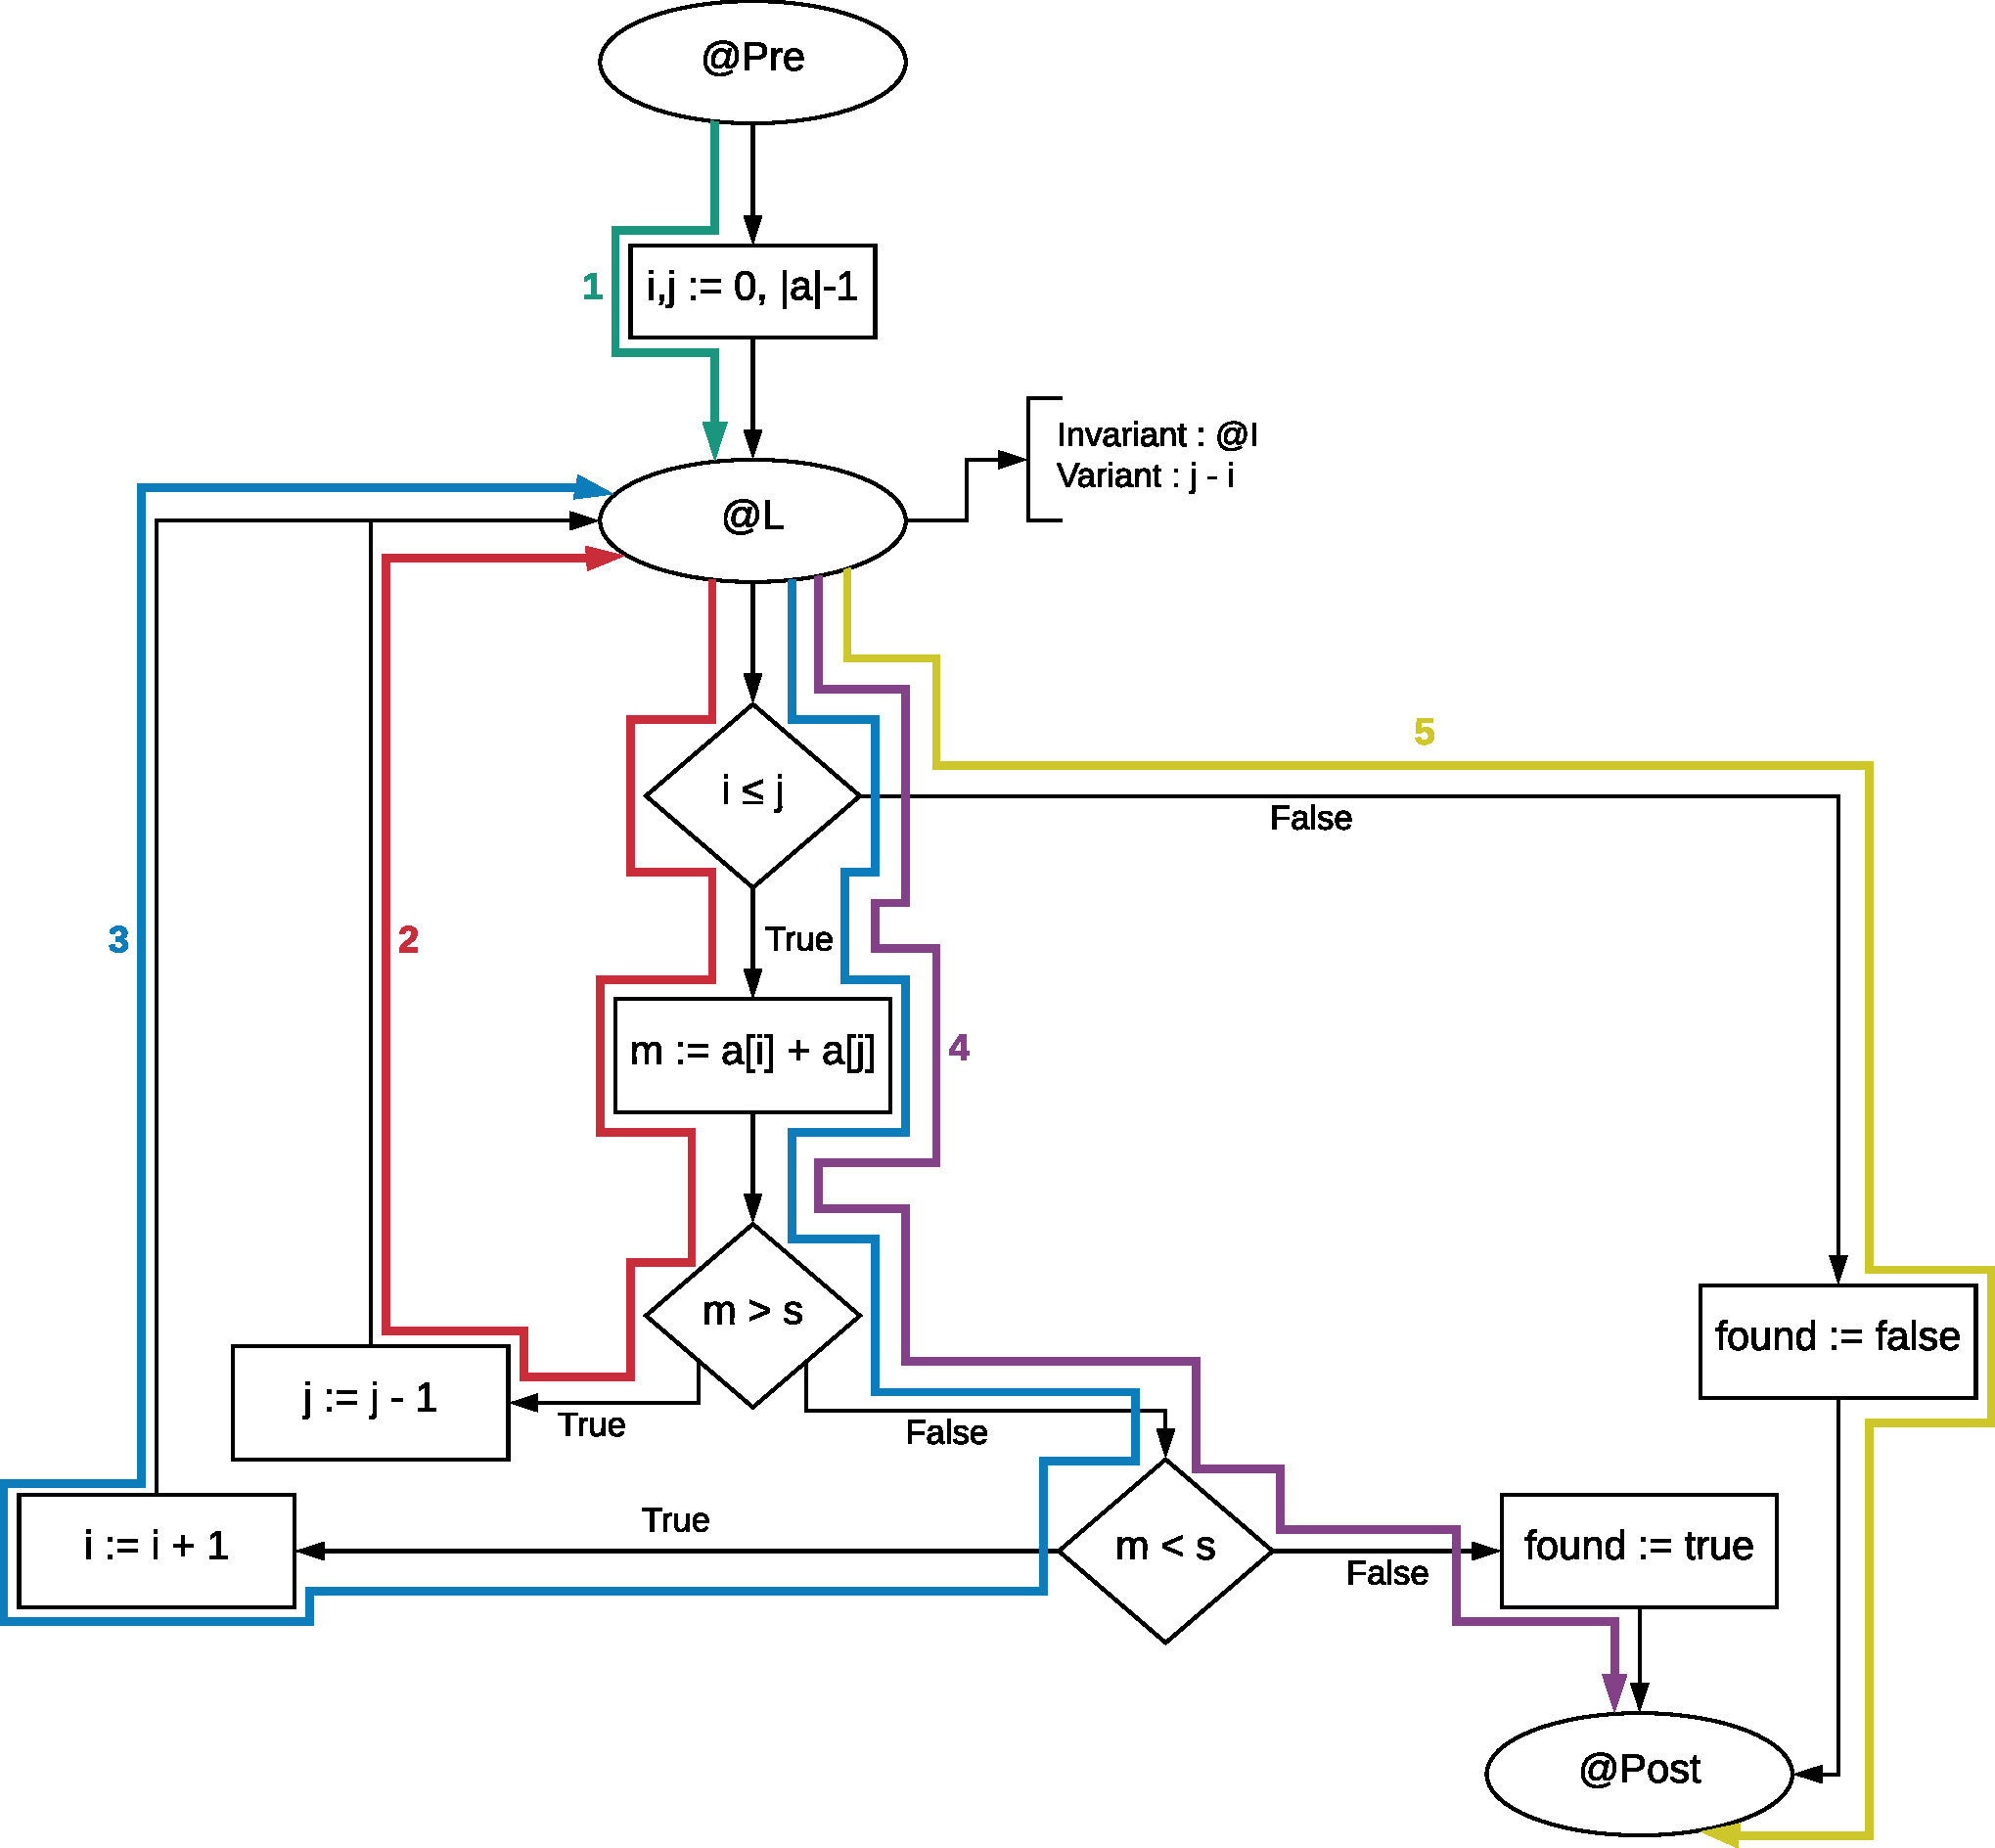
\includegraphics[width=\textwidth]{svg-inkscape/execgraph_svg-tex.pdf}
	\caption{Le graphe d'exécution complet pour le programme donné.}
	\label{fig:execgraph}
\end{figure}
Afin de faciliter les preuves, chaque chemin simple est redessiné à coté de sa preuve de correction.
Le point de coupe se trouve à l'entrée de la boucle.

\section{Preuve de correction partielle}
\label{sec:graph}
Avant de prouver la correction des différents chemins simples, définissons quelques prédicats:
\begin{align*}
&\begin{array}{l} \phantom{{} \land {}}\textnormal{\inlinedafny{sorted}}(a) \equiv \forall k, \ell \mid 0 \le k \le \ell < \abs{a} :: a[k] \le a[\ell]\end{array} \tag{Pre} \label{eq:Pre}\\\\
&\begin{array}{l}
\phantom{{} \land {}} 0 \le i \le j+1 \le \abs{a} \\ {} \land \forall p, x \mid 0 \le p < i \land 0 \le x < \abs{a} :: a[p] + a[x] \ne s \\ {} \land \forall q, x \mid j < q < \abs{a} \land 0 \le x < \abs{a} :: a[x] + a[q] \ne s
\end{array}\tag{I} \label{eq:I}\\\\
&\begin{array}{l}
\phantom{{} \land \lnot} \textnormal{\inlinedafny{found}} \implies 0 \le i \le j < \abs{a} \land a[i] + a[j] = s \\ {} \land \lnot\textnormal{\inlinedafny{found}} \iff \forall m, n \mid 0 \le m \le n < \abs{a} :: a[m] + a[n] \ne s
\end{array}\tag{Post} \label{eq:Post}
\end{align*}
On a également démontré une équivalence logique souvent utilisée dans les preuves de correction (\ref{ann:om}).
\subsection{Précondition jusqu'à l'entrée de la boucle}
\noindent\begin{minipage}[c]{0.35\textwidth}
\centering
\begin{figure}[H]
	\centering
	\includesvg[width=0.6\textwidth]{simplepath1}
	\caption{@\ref{eq:Pre} $\to$ @\ref{eq:I}.}
	\label{fig:1}
\end{figure}
\end{minipage}%
\begin{minipage}[c]{0.65\textwidth}
\begin{proof}
\begin{align*}
&\Big[\textnormal{\ref{eq:Pre}} \Big] \\
&\Big[0 \le 0 \le \abs{a} - 1 +1 \le \abs{a} \\
&\land \forall p, x \mid 0 \le p < 0 \land 0 \le x < \abs{a} :: a[p] + a[x] \ne s \\
&\land \forall q, x \mid \abs{a} - 1 < q < \abs{a} \land 0 \le x < \abs{a} :: a[x] + a[q] \ne s\Big] \\
&\textnormal{\inlinedafny{i, j := 0, |a| - 1;}} \\
&\Big[\textnormal{\ref{eq:I}} \Big]
\end{align*}
Afin d'affirmer la correction de ce chemin simple, on doit encore prouver que le deuxième prédicat est bien une conséquence de la précondition.
On peut simplifier ce deuxième prédicat pour montrer qu'il est en fait équivalent à $\top$.
Il est donc toujours impliqué par la précondition.
\end{proof}
\end{minipage}
\subsection{Boucle dans le cas $m > s$}
\noindent\begin{minipage}[c]{0.35\textwidth}
\centering
\begin{figure}[H]
	\centering
	\includesvg[width=0.6\textwidth]{simplepath2}
	\caption{@\ref{eq:I} $\to$ @\ref{eq:I} pour $m > s$.}
	\label{fig:2}
\end{figure}
\end{minipage}%
\begin{minipage}[c]{0.65\textwidth}
\begin{proof}
\begin{align*}
&\Big[\textnormal{\ref{eq:I}} \Big] \\
&\Big[i \le j \implies \big(a[i] + a[j] > s \implies \textnormal{I}_2\big) \Big] \\
&\textnormal{\inlinedafny{assume i <= j;}} \\
&\Big[a[i] + a[j] > s \implies \textnormal{I}_2 \Big] \\
&\textnormal{\inlinedafny{m := a[i] + a[j];}} \\
&\Big[m > s \implies \textnormal{I}_2 \Big] \\
&\textnormal{\inlinedafny{assume m > s;}} \\
&\Big[\textnormal{I}_2\Big] \equiv \Big[0 \le i \le j \le \abs{a} \\
&\land \forall p, x \mid 0 \le p < i \land 0 \le x < \abs{a} :: a[p] + a[x] \ne s \\
&\land \forall q, x \mid j-1 < q < \abs{a} \land 0 \le x < \abs{a} :: a[x] + a[q] \ne s \Big] \\
&\textnormal{\inlinedafny{j := j - 1;}} \\
&\Big[\textnormal{\ref{eq:I}} \Big]
\end{align*}
Pour montrer que l'invariant implique bien le deuxième prédicat,
on doit prouver que
\begin{align*}
&\Big(\textnormal{\ref{eq:I}} \implies \Big[i \le j \implies \big(a[i] + a[j] > s \implies \textnormal{I}_2\big) \Big]\Big) \\
\equiv &\Big[\textnormal{\ref{eq:I}} \land i \le j \land a[i] + a[j] > s\Big] \implies \textnormal{I}_2\,.
\end{align*}
Pour ne pas trop surcharger les équations, on procède partie par partie.
Dans l'invariant \ref{eq:I}, la première partie de la conjonction permet d'obtenir $0 \le i \le j \le \abs{a}$,
car $(i \le j+1) \land (i \le j) \implies i \le j$.
La deuxième partie de la conjonction est exactement la même dans \ref{eq:I} et I$_2$,
et ne nécessite donc pas de développement.
Pour la troisième partie, elle est identique sauf dans le cas $q = j$.
Dans ce cas, comme on a également que $a[i] + a[j] > s$,
et que le tableau est trié, le seul moyen d'obtenir $a[i] + a[j] = s$ avec $a[j]$ fixé serait de prendre un élément $a[p] < a[i]$, avec donc $0 \le p < i$, comme le tableau est trié.
Or, par la deuxième partie de la conjonction de l'invariant, on sait que $\forall p, x \mid 0 \le p < i \land 0 \le x < \abs{a} :: a[p] + a[x] \ne s$.
Dans notre cas de figure, il suffit de prendre $x = j$ pour prouver qu'on n'aura jamais $a[p] + a[j] = s$ pour $0 \le p < i$.
\end{proof}
\end{minipage}

\subsection{Boucle dans le cas $m < s$}
\noindent\begin{minipage}[c]{0.35\textwidth}
\centering
\begin{figure}[H]
	\centering
	\includesvg[width=0.6\textwidth]{simplepath3}
	\caption{@\ref{eq:I} $\to$ @\ref{eq:I} pour $m < s$.}
	\label{fig:3}
\end{figure}
\end{minipage}%
\begin{minipage}[c]{0.65\textwidth}
\begin{proof}
\begin{align*}
&\Big[\textnormal{\ref{eq:I}} \Big] \\
&\Big[i \le j \implies \big(a[i] + a[j] < s \implies \textnormal{I}_3\big) \Big] \\
&\textnormal{\inlinedafny{assume i <= j;}} \\
&\Big[a[i] + a[j] < s \implies \textnormal{I}_3 \Big] \\
&\textnormal{\inlinedafny{m := a[i] + a[j];}} \\
&\Big[\big(\lnot(m > s) \implies (m < s \implies \textnormal{I}_3)\big)\Big] \equiv \Big[\big(m < s \implies \textnormal{I}_3\big)\Big] \\
&\textnormal{\inlinedafny{assume !(m > s);}} \\
&\Big[m < s \implies \textnormal{I}_3 \Big] \\
&\textnormal{\inlinedafny{assume m < s;}} \\
&\Big[\textnormal{I}_3\Big] \equiv \Big[0 \le i + 1 \le j + 1 \le \abs{a} \\
&\land \forall p, x \mid 0 \le p < i + 1 \land 0 \le x < \abs{a} :: a[p] + a[x] \ne s \\
&\land \forall q, x \mid j < q < \abs{a} \land 0 \le x < \abs{a} :: a[x] + a[q] \ne s \Big] \\
&\textnormal{\inlinedafny{i := i +1;}}\\
&\Big[\textnormal{\ref{eq:I}} \Big]
\end{align*}
Pour montrer que l'invariant implique bien le deuxième prédicat,
on doit prouver que
\begin{align*}
&\Big(\textnormal{\ref{eq:I}} \implies \Big[i \le j \implies \big(a[i] + a[j] < s \implies \textnormal{I}_3\big) \Big]\Big) \\
\equiv &\Big[\textnormal{\ref{eq:I}} \land i \le j \land a[i] + a[j] < s\Big] \implies \textnormal{I}_3\,.
\end{align*}
Pour ne pas trop surcharger les équations, on procède partie par partie.
Dans l'invariant \ref{eq:I}, la première partie de la conjonction permet d'obtenir $0 \le i +1 \le j+1 \le \abs{a}$,
car $(i \le j+1) \land (i \le j) \implies i+1 \le j+1$.
La troisième partie de la conjonction est exactement la même dans \ref{eq:I} et I$_3$,
et ne nécessite donc pas de développement.
Pour la deuxième partie, elle est identique sauf dans le cas $p = i$.
Dans ce cas, comme on a également que $a[i] + a[j] < s$,
et que le tableau est trié, le seul moyen d'obtenir $a[i] + a[j] = s$ avec $a[i]$ fixé serait de prendre un élément $a[q] > a[j]$, avec donc $j  < q < \abs{a}$, comme le tableau est trié.
Or, par la troisième partie de la conjonction de l'invariant, on sait que $\forall q, x \mid j < q < \abs{a} \land 0 \le x < \abs{a} :: a[x] + a[q] \ne s$.
Dans notre cas de figure, il suffit de prendre $x = i$ pour prouver qu'on n'aura jamais $a[i] + a[q] = s$ pour $j < q < \abs{a}$.
\end{proof}
\end{minipage}

\subsection{Entrée de la boucle jusqu'à la sortie dans le cas $a[i] + a[j] = s$}
\noindent\begin{minipage}[c]{0.35\textwidth}
\centering
\begin{figure}[H]
	\centering
	\includesvg[width=0.6\textwidth]{simplepath4}
	\caption{@\ref{eq:I} $\to$ @\ref{eq:Post} pour $a[i] + a[j] = s$.}
	\label{fig:4}
\end{figure}
\end{minipage}%
\begin{minipage}[c]{0.65\textwidth}
\begin{proof}
\begin{align*}
&\Big[\textnormal{\ref{eq:I}} \Big] \\
&\Big[i \le j \implies \big(a[i] + a[j] = s \implies  \textnormal{Post}_2  \big) \Big] \\
&\textnormal{\inlinedafny{assume i <= j;}} \\
&\Big[a[i] + a[j] = s \implies  \textnormal{Post}_2 \Big] \\
&\textnormal{\inlinedafny{m := a[i] + a[j];}} \\
&\Big[\lnot (m > s) \implies \big(\lnot (m < s) \implies  \textnormal{Post}_2  \big)\Big] \equiv \Big[(m = s) \implies  \textnormal{Post}_2 \Big] \\
&\textnormal{\inlinedafny{assume !(m>s);}} \\
&\Big[\lnot (m < s) \implies \textnormal{Post}_2 \Big] \\
&\textnormal{\inlinedafny{assume !(m<s);}} \\
&\Big[\textnormal{Post}_2 \Big] \equiv \Big[\top \implies 0 \le i \le j < \abs{a} \land a[i] + a[j] = s \\
&\land \lnot \top \iff \forall m, n \mid 0 \le m \le n < \abs{a} :: a[m] + a[n] \ne s \Big] \\
&\textnormal{\inlinedafny{found := true;}} \\
&\Big[\textnormal{\ref{eq:Post}}\Big]
\end{align*}
Pour montrer que l'invariant implique bien le deuxième prédicat,
on doit prouver que
\begin{align*}
&\Big(\textnormal{\ref{eq:I}} \implies \Big[i \le j \implies \big(a[i] + a[j] = s \implies \textnormal{Post}_2\big) \Big]\Big) \\
\equiv &\Big[\textnormal{\ref{eq:I}} \land i \le j \land a[i] + a[j] = s\Big] \implies \textnormal{Post}_2\,.
\end{align*}
Pour ne pas trop surcharger les équations, on procède partie par partie.
Dans l'invariant \ref{eq:I}, la première partie de la conjonction permet d'obtenir $0 \le i \le j < \abs{a}$,
car $(i \le j+1) \land (i \le j) \equiv i \le j$ et $j+1 \le \abs{a} \implies j < \abs{a}$.
Le prédicat Post$_2$ peut être réécrit comme
\begin{align*}
\textnormal{Post}_2 \equiv&\,\Big(0 \le i \le j < \abs{a} \land a[i] + a[j] = s\Big)\\
\land&\,\Big(\exists m, n \mid 0 \le m \le n < \abs{a} :: a[m] + a[n] = s\Big)\,.
\end{align*}
On voit donc que la condition $a[i] + a[j] = s$ réapparaît également.
Finalement, on prend le cas $m = i$, $n = j$, ce qui représente la deuxième partie de Post$_2$.
 On a donc bien prouvé que la plus faible précondition de ce tableau est une conséquence de l'invariant.
\end{proof}
\end{minipage}

\subsection{Entrée de la boucle jusqu'à la sortie dans le cas $a[i] + a[j] \ne s$}
\noindent\begin{minipage}[c]{0.35\textwidth}
\centering
\begin{figure}[H]
	\centering
	\includesvg[width=0.6\textwidth]{simplepath5}
	\caption{@\ref{eq:I} $\to$ @\ref{eq:Post} pour $a[i] + a[j] \ne s$.}
	\label{fig:5}
\end{figure}
\end{minipage}%
\begin{minipage}[c]{0.65\textwidth}
\begin{proof}
\begin{align*}
&\Big[\textnormal{\ref{eq:I}} \Big] \\
&\Big[\lnot(i \le j) \implies \textnormal{Post}_3 \Big] \equiv \Big[i > j \implies \textnormal{Post}_3 \Big] \\
&\textnormal{\inlinedafny{assume !(i <= j);}} \\
&\Big[\textnormal{Post}_3 \Big] \equiv \Big[\bot \implies 0 \le i \le j < \abs{a} \land a[i] + a[j] = s \\
&\land \lnot \bot \iff \forall m, n \mid 0 \le m \le n < \abs{a} :: a[m] + a[n] \ne s \Big] \\
&\textnormal{\inlinedafny{found := false;}} \\
&\Big[\textnormal{\ref{eq:Post}}\Big]
\end{align*}
Pour montrer que l'invariant implique bien le deuxième prédicat,
on doit prouver que
\begin{align*}
&\Big(\textnormal{\ref{eq:I}} \implies \Big[i > j \implies \textnormal{Post}_3 \Big]\Big) \\
\equiv &\Big[\textnormal{\ref{eq:I}} \land i > j \Big] \implies \textnormal{Post}_3\,.
\end{align*}
Pour ne pas trop surcharger les équations, on procède partie par partie.
Dans l'invariant \ref{eq:I}, la première partie de la conjonction permet d'obtenir $j < i \le j + 1 \le \abs{a}$, et donc $i = j + 1$.
On peut alors réécrire l'invariant (qui est en réalité devenu $\textnormal{\ref{eq:I}} \land i > j$) comme
\begin{align*}
&{-1} \le j < i = j+1 \le \abs{a} \\
\land\,&\forall p, x \mid 0 \le p < j+1 \land 0 \le x < \abs{a} :: a[p] + a[x] \ne s \\
\land\,&\forall q, x \mid j < q < \abs{a} \land 0 \le x < \abs{a} :: a[x] + a[q] \ne s \\
\equiv\,& {-1} \le j < i = j+1 \le \abs{a} \\
\land\,&\forall x, y \mid 0 \le y < \abs{a} \land 0 \le x < \abs{a} :: a[x] + a[y] \ne s\,.
\end{align*}
On réécrit aussi le prédicat Post$_3$, comme suit:
\[
\textnormal{Post}_3 \equiv \Big(\forall m, n \mid 0 \le m \le n < \abs{a} :: a[m] + a[n] \ne s\Big)\,.
\]
On remarque bien que $\textnormal{\ref{eq:I}} \land i > j \implies \textnormal{Post}_3$,
ce qui conclut la preuve.
\end{proof}
\end{minipage}
\section{Preuve de terminaison}
\label{sec:term}
Afin de montrer que le programme se termine, il faut montrer que le variant diminue à chaque itération.
On choisit ici le variant $j-i+1$ (pour qu'il soit toujours positif ou nul).
Pour faire ceci, on distingue trois cas:
\begin{itemize}
	\item la valeur de $a[i] + a[j] = m > s$;
	\item la valeur de $a[i] + a[j] = m < s$;
	\item la valeur de $a[i] + a[j] = m = s$.
\end{itemize}
Dans les deux premiers cas, on démontre relativement facilement que le variant diminue d'une unité à chaque itération, alors que dans le troisième cas, le programme se termine immédiatement, peu importe la valeur du variant.
On se limitera donc à la preuve des deux premiers cas.
Comme montré au cours, il faudra donc pour chaque chemin simple $@L_i'S@L_j'$ prouver $[P_i \land V_i = v_0]\ S\ [V_j < v_0]$.
\subsection{Évolution du variant dans le cas $m > s$}
\begin{proof}
Dans ce cas, montré à la \textsc{Figure}~\ref{fig:2},
l'évolution du variant au cours de l'exécution est ajoutée aux tableau d'assertions déjà donné.
\begin{align*}
&\Big[j - i  + 1 = V_0 \land \textnormal{\ref{eq:I}} \Big] \\
&\Big[i \le j \implies \big(a[i] + a[j] > s \implies j - i < V_0\big) \Big] \\
&\textnormal{\inlinedafny{assume i <= j;}} \\
&\Big[a[i] + a[j] > s \implies j - i < V_0 \Big] \\
&\textnormal{\inlinedafny{m := a[i] + a[j];}} \\
&\Big[m > s \implies j - i < V_0 \Big] \\
&\textnormal{\inlinedafny{assume m > s;}} \\
&\Big[j - 1 - i + 1 < V_0  \Big] \\
&\textnormal{\inlinedafny{j := j - 1;}} \\
&\Big[j - i + 1 < V_0 \Big]
\end{align*}
On a bien $(j - i + 1)_\textnormal{initial} > (j - i + 1)_\textnormal{final}$. On trouve donc bien que le variant à la sortie de la boucle est strictement plus petit que le variant en entrée.
Comme on sait que la valeur minimale du variant est atteinte lorsque $i = j+1 \implies j - i + 1 = 0$ (on a en fait $j - i + 1 \ge 0$),
le programme doit se terminer après un nombre fini d'étapes.
\end{proof}

\subsection{Évolution du variant dans le cas $m < s$}
\begin{proof}
Dans ce cas, montré à la \textsc{Figure}~\ref{fig:3},
l'évolution du variant au cours de l'exécution est ajoutée aux tableau d'assertions déjà donné.
\begin{align*}
&\Big[j - i + 1 = V_0 \land \textnormal{\ref{eq:I}} \Big] \\
&\Big[i \le j \implies \big(a[i] + a[j] < s \implies j - i < V_0\big) \Big] \\
&\textnormal{\inlinedafny{assume i <= j;}} \\
&\Big[a[i] + a[j] < s \implies j - i < V_0 \Big] \\
&\textnormal{\inlinedafny{m := a[i] + a[j];}} \\
&\Big[\big(\lnot(m > s) \implies (m < s \implies j - i < V_0\big) \Big] \equiv \Big[m < s \implies j - i < V_0 \Big]\\
&\textnormal{\inlinedafny{assume !(m > s);}} \\
&\Big[m < s \implies j - i < V_0 \Big] \\
&\textnormal{\inlinedafny{assume m < s;}} \\
&\Big[j - (i + 1) + 1 < V_0 \Big]\\ % On peut pas changer en = !!!, on doit juste remplacer par les diff valeurs, pas mettre =
&\textnormal{\inlinedafny{i := i + 1;}} \\
&\Big[j - i + 1 < V_0 \Big]% on ne met pas le I, cf. slide 55 CM4 ou même 47 ou c'est formellement mis.
\end{align*}
On a bien $(j - i + 1)_\textnormal{initial} > (j - i + 1)_\textnormal{final}$. On trouve donc bien que le variant à la sortie de la boucle est strictement plus petit que le variant en entrée.
Comme on sait que la valeur minimale du variant est atteinte lorsque $i = j+1 \implies j - i + 1 = 0$ (on a en fait $j - i + 1 \ge 0$),
le programme doit se terminer après un nombre fini d'étapes.
\end{proof}

\section{Conclusion}
Comme nous avons prouvé à la \textsc{Section}~\ref{sec:graph} que les différents chemins d'exécution sont corrects, et que nous avons prouvé à la \textsc{Section}~\ref{sec:term} que le programme se termine après un nombre fini d'étapes, on a ainsi prouvé la correction totale de l'algorithme.

C'est grâce à la garantie de diminution du variant d'ailleurs qu'il est possible d'affirmer que le temps d'exécution de l'algorithme est linéaire en la taille de la séquence d'entiers.

\appendix
\section{Preuve omise}
\label{ann:om}
On montre ici que $A \implies B \implies C \equiv A \land B \implies C$.
\begin{proof}
\begin{align*}
A \implies B \implies C &\equiv \lnot A \lor (B \implies C) \\
&\equiv \lnot A \lor (\lnot B \lor C) \\
&\equiv \lnot A \lor \lnot B \lor C \\
&\equiv \lnot(A \land B) \lor C \\
&\equiv A \land B \implies C\,.\qedhere
\end{align*}
\end{proof}
\end{document}
